\documentclass[11pt]{article}
\usepackage[margin=1in]{geometry}
\usepackage{booktabs}
\usepackage{graphicx}
\usepackage{amsmath}
\usepackage{xcolor}
\usepackage{microtype}
\usepackage[colorlinks=true,linkcolor=blue!50!black,citecolor=blue!50!black,urlcolor=blue!50!black]{hyperref}
\usepackage{titlesec}
\titlespacing{\section}{0pt}{1.4ex plus 1ex minus .2ex}{0.8ex}
\titlespacing{\subsection}{0pt}{1.0ex plus 1ex minus .2ex}{0.5ex}

\newcommand{\code}[1]{\texttt{\small #1}}

\title{\textbf{What and How Does the Translation Task Work Inside an LLM?}\\[2pt]
\large An interpretability study across eight multilingual models, and what it
implies for quantization}
\author{Arctos project --- Phase One findings report}
\date{2026-05-28}

\begin{document}
\maketitle

\begin{abstract}
\noindent
We investigate \emph{how} eight open multilingual language models carry out
machine translation, using five complementary interpretability methods on a
single uniform hooking framework, and a sixth purpose-built ``language-pivot''
analysis aimed squarely at the title question. Across decoder-only models
spanning four lineages, two normalizations, two positional encodings, and
2022--2025 generations --- plus one encoder--decoder (NLLB) --- a consistent
mechanistic picture emerges: translation is computed as a depth-ordered
pipeline (source encoding $\rightarrow$ a language-agnostic / pivot
representation in the middle $\rightarrow$ target-language commitment in the
final layers), and the \emph{relative depth} of this pipeline generalizes
across architectures with a single clean exception (Gemma-family). We also
report a negative result that matters for compression: component
\emph{importance} (where the MT work concentrates) does \emph{not} predict
quantization \emph{sensitivity} (where numerical precision matters),
confirmed across two independent metrics. We close with what this means for an
interpretability-guided quantization method.
\end{abstract}

\section{The question, and how we attack it}

The title question --- \emph{what and how does translation work in an LLM?}
--- is mechanistic: not ``how well does it translate'' but ``what internal
computation produces the translation, and where in the network does each part
happen.'' We answer it by reading and intervening on the \textbf{residual
stream}, the additive running sum that flows down a transformer:
\[
\text{resid}_\ell = \text{embed} + \sum_{\ell' \le \ell}\bigl(\text{attn\_out}_{\ell'} + \text{mlp\_out}_{\ell'}\bigr).
\]
Every method below either \emph{reads} this stream (logit lens, probing,
pivot trajectory), \emph{decomposes} it into per-component contributions
(IFR, DLA), or \emph{intervenes} on it causally (attribution patching, noise
injection). A single wrapper (\code{HookedModel}) exposes a uniform interface
---\code{run\_with\_cache}, \code{W\_U}, \code{W\_O}, \code{ln\_final}---
across all architectures, so the same method code runs on Cohere, Llama,
Gemma, BLOOM, and (with a dedicated path) the NLLB encoder--decoder.

\section{Setup}

\paragraph{Models.} Eight models chosen to span training intent, architecture
family, and generation (Table~\ref{tab:models}). The TowerBase\,$\rightarrow$\,
TowerInstruct pair is a controlled ablation isolating MT-task supervised
fine-tuning (SFT); both build on a continued-pretraining (CPT) base.

\paragraph{Data.} FLORES+ dev, three language pairs chosen for contrast:
\textbf{cs$\rightarrow$de} (same script, sanity pair), \textbf{en$\rightarrow$zh}
(cross-script, Han target), \textbf{en$\rightarrow$arz} (cross-script, Egyptian
Arabic --- a low-resource, non-standard variety). 200 sentences/pair for the
correlational methods; fewer for the generation-heavy causal ones.

\begin{table}[t]\centering\small
\begin{tabular}{llll}
\toprule
Model & Year & Architecture & Training intent \\
\midrule
Aya Expanse 8B & 2024 & Cohere, RoPE, RMSNorm & general multilingual LM \\
TowerBase 7B & 2024 & Llama-2 & + bilingual CPT (no SFT) \\
TowerInstruct 7B & 2024 & Llama-2 & + MT-task SFT \\
Tower-Plus 9B & 2025 & \textbf{Gemma 2} & CPT + MT-SFT \\
BLOOM 7B1 & 2022 & \textbf{ALiBi, LayerNorm} & multilingual pretraining \\
EuroLLM 9B & 2024 & Llama-3 & European MT specialist \\
Llama-3.1 8B & 2024 & Llama-3, GQA & general LM \\
Gemma-3 12B & 2025 & Gemma 3 & baseline (Google QAT) \\
\midrule
NLLB-200 3.3B & 2022 & \textbf{encoder--decoder} & MT-purpose-built \\
\bottomrule
\end{tabular}
\caption{The model set. Bold marks the architectural outliers that test
generalization.}
\label{tab:models}
\end{table}

\section{The methods, and what each reveals}

\paragraph{Logit lens.} Apply the model's own final norm + unembedding to an
\emph{intermediate} residual: $\text{logits}_\ell = \text{LN}_f(\text{resid}_\ell)\,W_U$.
This reads ``what would the model predict if it had to decide at layer
$\ell$.'' Tracking the probability mass on the gold target tokens across
layers shows \emph{when} the model commits to the translation. (Invariant we
verify: at the last layer the lens equals the model's real logits, to
$<\!10^{-4}$.)

\paragraph{Probing.} Train a linear classifier per layer to predict a feature
(source/target language) from the residual; report \emph{selectivity} =
accuracy $-$ control-task accuracy (Hewitt \& Liang 2019), which separates
``the feature is represented'' from ``the probe memorized.'' Reveals
\emph{where} language identity becomes linearly decodable.

\paragraph{Information Flow Routes (IFR).} Decompose the residual into
per-component contributions and take their $L_1$-normalized magnitudes:
$\text{IFR}(c)=\lVert c\rVert_1 / \sum_{c'}\lVert c'\rVert_1$, averaged over
the set. Unsigned; tells you which components are \emph{loud}. Reveals
\emph{where} (which layers/heads) MT computation concentrates.

\paragraph{Direct logit attribution (DLA).} Decompose the \emph{target-token
logit} into signed per-component contributions via the norm-linearized
unembed: $\text{DLA}(c)=(c\odot s)\cdot W_U[:,t]$. Signed: positive = pushes
toward the target token (a ``predictor''), negative = away (a
``suppressor''). Reveals \emph{which} components are causally aimed at the
right output token.

\paragraph{Attribution patching (causal).} First-order approximation of
activation patching: $\text{effect}(c)\approx \partial L/\partial a_c \cdot
(a_c^{\text{corrupt}}-a_c^{\text{clean}})$. One backward pass scores every
component. Reveals which components, if damaged, \emph{break} the translation.

\paragraph{Noise sensitivity (quantization proxy).} Add relative Gaussian
noise to a component's weights and measure the resulting quality drop ---
directly simulating quantization error. Reveals where numerical
\emph{precision} matters.

\paragraph{Language-pivot trajectory (the ``how'' centerpiece).} For
cross-script pairs the target uses a different writing system from
English/source (Han for zh, Arabic for arz, vs.\ Latin). We logit-lens each
layer and classify the script of the top-50 tokens, measuring the share of
probability mass on Latin vs.\ target script vs.\ other. If the model
``thinks in English/source'' mid-stack and converts to the target script
late, the trajectory shows Latin dominance giving way to target script in the
final layers --- the mechanistic signature of pivot-based translation
(cf.\ Wendler et al.\ 2024).

\section{Findings: what and how}

\subsection{Translation is a depth-ordered pipeline}

Three methods agree on the coarse structure. \textbf{(1) Source language} is
linearly decodable from very early --- typically the embedding (L0) for
heavily multilingually-trained models and mid-network (L9--L17) for
general-LM-style models (Table~\ref{tab:q1}), but present at 0.4--0.55
selectivity at \emph{every} layer. \textbf{(2) Target commitment} (logit-lens
mass on the gold target tokens) stays near zero through the first half and
rises only in the final layers (Fig.~\ref{fig:lens}). \textbf{(3) Computation
magnitude} (IFR) concentrates in the last quarter of depth
(Fig.~\ref{fig:ifr}). The picture: \emph{understand the source early, do the
cross-lingual work in the middle, commit to the target late.}

\begin{table}[t]\centering\small
\begin{tabular}{lccc}
\toprule
Model & source-ID peak layer (sel.) & IFR 1st-quarter & IFR last-quarter \\
\midrule
Aya Expanse 8B & L17 (0.55) & 8\% & 56\% \\
TowerBase 7B & L0 (0.60) & 6\% & 45\% \\
TowerInstruct 7B & L0 (0.56) & 6\% & 46\% \\
BLOOM 7B1 & L0 (0.55) & 12\% & 44\% \\
EuroLLM 9B & L9 (0.54) & 2\% & 52\% \\
Llama-3.1 8B & L0 (0.55) & 8\% & 47\% \\
NLLB-200 3.3B (decoder) & --- & 12\% & 45\% \\
\midrule
\textbf{Tower-Plus 9B (Gemma 2)} & L7 (0.54) & \textbf{32\%} & \textbf{17\%} \\
\textbf{Gemma-3 12B} & L29 (0.59) & \textbf{92\%} & \textbf{3\%} \\
\bottomrule
\end{tabular}
\caption{Q1/Q4 depth structure. Six decoder-only models \emph{and} the NLLB
encoder--decoder share the profile (first quarter light, last quarter
dominant). Both Gemma-family models invert it --- an architecture artifact of
Gemma's extra per-layer norms + logit soft-capping.}
\label{tab:q1}
\end{table}

\begin{figure}[t]\centering

\includegraphics[width=0.78\linewidth]{figures/lens_combined.png}
\caption{Logit-lens target-token mass vs.\ depth fraction, all models, all
pairs. Mass is near zero through mid-depth and rises late --- target-language
commitment is a late-layer event.}
\label{fig:lens}
\end{figure}

\begin{figure}[t]\centering

\includegraphics[width=0.92\linewidth]{figures/ifr_depth_partition.png}
\caption{IFR contribution share by depth quarter. Last-quarter dominance is
consistent across lineages, normalizations, positional encodings, and the
decoder-only/enc--dec divide --- the lone exceptions are the two
Gemma-family models.}
\label{fig:ifr}
\end{figure}

\subsection{How the cross-lingual step works: the pivot trajectory}
\label{sec:pivot}

This is the most direct evidence for \emph{how} translation happens. For the
cross-script pairs we measure, per layer, the share of the top-50 lens
tokens' probability mass on the target script (Han / Arabic) versus Latin
(English/source). The result is unambiguous (Table~\ref{tab:pivot},
Fig.~\ref{fig:pivot}): \textbf{target-script mass is essentially zero through
the first $\sim$80--95\% of depth, then rises sharply in the final layers.}
The model represents the in-progress translation in a Latin/pivot space ---
not the target script --- for almost the entire forward pass, and converts to
the target writing system only at the very end.

\begin{table}[t]\centering\small
\begin{tabular}{lcccc}
\toprule
Model (en$\rightarrow$zh) & tgt-script @ L0 & @ mid-depth & @ last & Latin$\rightarrow$tgt crossover \\
\midrule
Aya Expanse 8B & 0.00 & 0.44 & 0.87 & depth 0.50 \\
EuroLLM 9B & 0.00 & 0.00 & 0.83 & depth 0.60 \\
Tower-Plus 9B & 0.00 & 0.00 & 0.56 & depth 0.95 \\
Llama-3.1 8B & 0.00 & 0.00 & 0.41 & depth 0.97 \\
Gemma-3 12B & 0.00 & 0.00 & 0.72 & depth 0.96 \\
BLOOM 7B1 & 0.00 & 0.00 & 0.61 & never $>$ Latin \\
\bottomrule
\end{tabular}
\caption{Language-pivot trajectory, en$\rightarrow$zh. Target-script (Han)
probability mass under the logit lens is near zero until late depth; the
crossover where target script overtakes Latin happens in the final layers
(depth fraction $\ge 0.9$ for most models). Aya, the strongest general
multilingual model, commits earliest (depth 0.50). This is the signature of
``process in a pivot/English-aligned space, emit in the target language
last.''}
\label{tab:pivot}
\end{table}

\begin{figure}[t]\centering
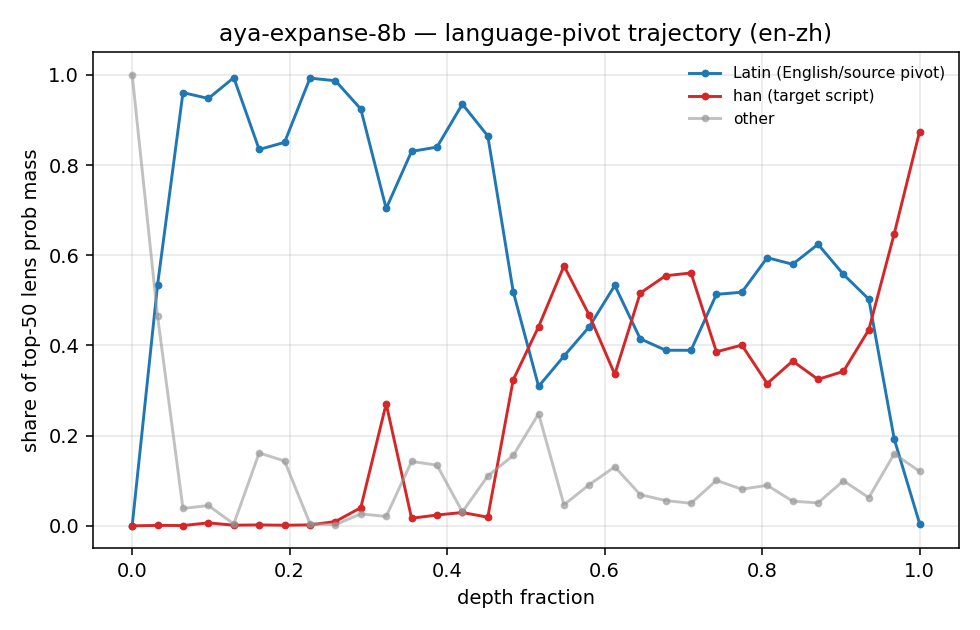
\includegraphics[width=0.49\linewidth]{figures/pivot_aya_enzh.png}\hfill
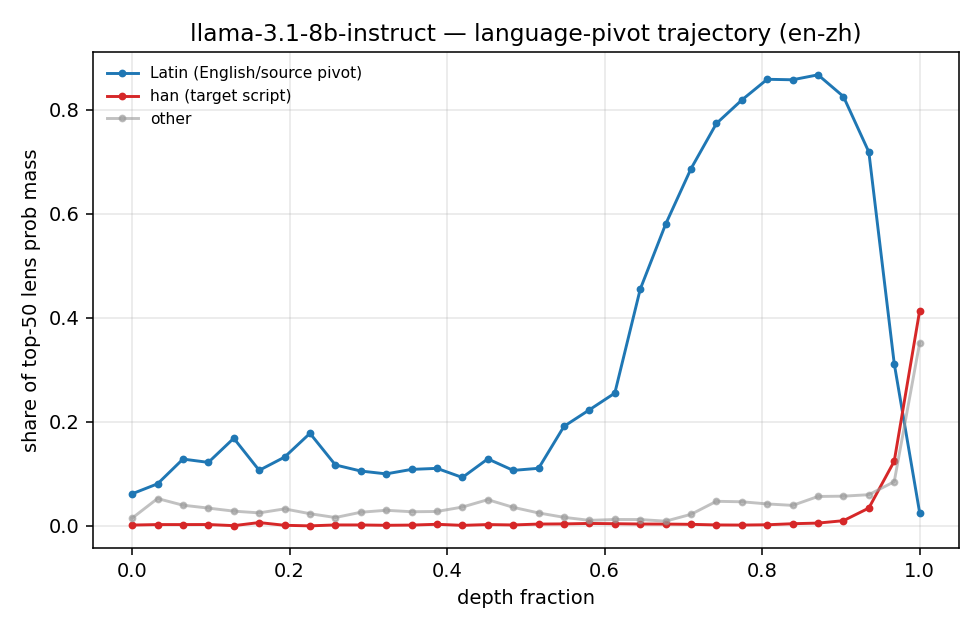
\includegraphics[width=0.49\linewidth]{figures/pivot_llama_enzh.png}
\caption{Pivot trajectories, en$\rightarrow$zh. Left: Aya (commits to Han
mid-stack). Right: Llama-3.1 (Latin/pivot dominant until the final layers,
then a sharp switch to Han). In both, the target script is absent for most of
the network --- the cross-lingual conversion is a late, localized event.}
\label{fig:pivot}
\end{figure}

The en$\rightarrow$arz pair tells the same story where the model can produce
Arabic at all (crossover at depth 0.81--0.97 for the capable models; weaker
models never cross, consistent with their low en$\rightarrow$arz quality).
This directly answers the ``how'': \emph{the middle of the network is not
working in the target language at all --- it operates in a
script-agnostic/pivot representation, and target-language identity is written
in only at the end}, exactly where the logit-lens target mass (Fig.~\ref{fig:lens}),
positive DLA (Fig.~\ref{fig:dla}), and IFR magnitude (Fig.~\ref{fig:ifr}) all
concentrate.

\subsection{Which components, and what they do (DLA + attention)}

DLA isolates recurring, pair-agnostic heads. In Aya, head L30.H8 is a strong
cross-pair \emph{predictor} (DLA $+0.72$ on cs$\rightarrow$de, $+0.44$ on
en$\rightarrow$arz); L29.H16 and L26.H5 are systematic \emph{suppressors}
(negative across pairs). The signed DLA depth curve
(Fig.~\ref{fig:dla}) shows the same late-commitment shape as the lens, now
direction-aware: positive contribution to the target token accumulates in the
last layers. Attention-pattern inspection of the top-DLA heads characterizes
what they do (source-attender / previous-token / sink); per-model role tables
are in \code{results/\{model\}/q2/attention/head\_roles.json}.

\begin{figure}[t]\centering
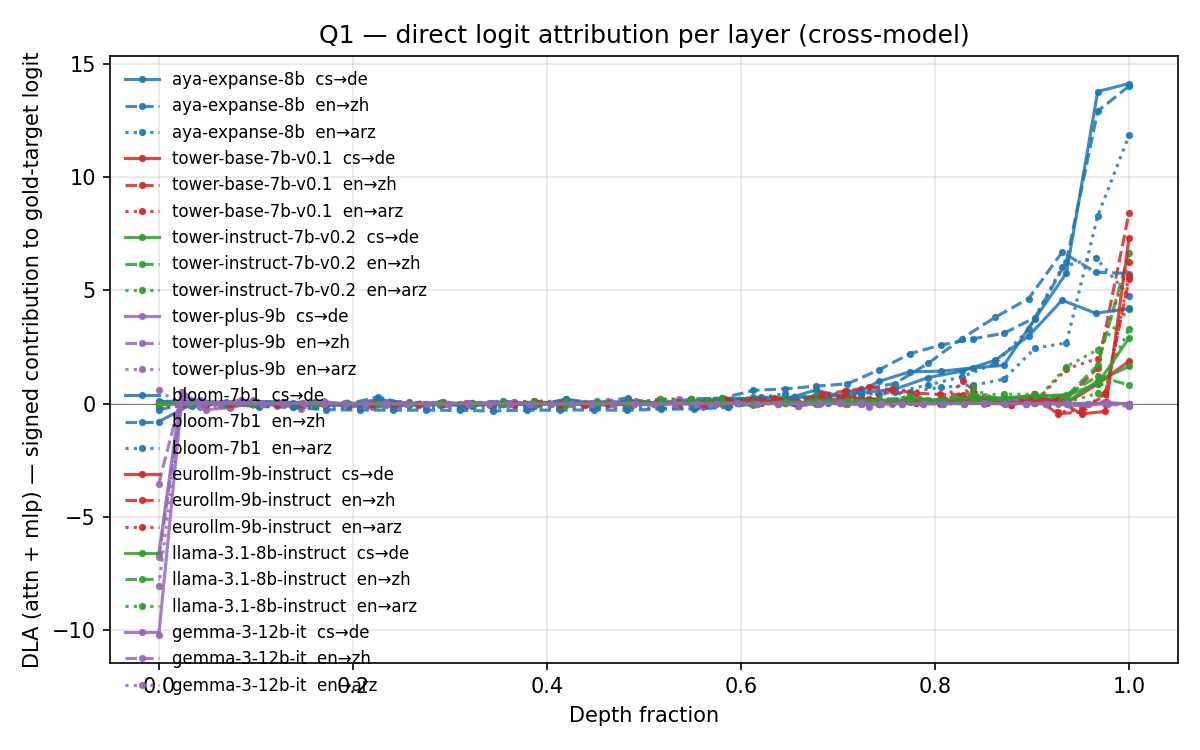
\includegraphics[width=0.78\linewidth]{figures/dla_layer_combined.png}
\caption{Signed direct logit attribution per layer. Positive
target-token contribution concentrates in the final layers; the Gemma-family
embedding spike (negative at L0) is the soft-capping artifact again.}
\label{fig:dla}
\end{figure}

\subsection{The MT footprint generalizes across architectures (Q4)}

The depth signature (Table~\ref{tab:q1}, Figs.~\ref{fig:lens}--\ref{fig:ifr})
holds across: two normalizations (RMSNorm, LayerNorm), two positional
encodings (RoPE, ALiBi), four lineages (Cohere, Llama, BigScience, EuroLLM),
2022$\rightarrow$2024 generations, \emph{and} the decoder-only
$\leftrightarrow$ encoder--decoder divide (NLLB's decoder matches). This
supports the strong form of the shared-depth hypothesis (a characteristic
relative-depth signature), with one boundary: \textbf{Gemma-family inverts
it}, so the signature is family-bounded, not universal.

\subsection{Importance does not predict quantization sensitivity (Q5)}

The components IFR/DLA flag as important are \emph{not} the ones where
quantization precision matters. Tested at two levels, both null
(Table~\ref{tab:q5}):

\begin{table}[t]\centering\small
\begin{tabular}{lccc}
\toprule
Experiment & perturbation & metric & mean $\rho$(importance, sensitivity) \\
\midrule
Per-head & one head's $W_O$ cols & target logit drop & $-0.025$ ($n{=}18$, $t{=}{-}0.55$) \\
Per-layer & whole layer's weights & \textbf{chrF++ drop} & $-0.065$ (IFR), $-0.046$ (DLA) \\
\bottomrule
\end{tabular}
\caption{Importance vs.\ sensitivity. The stronger per-layer/chrF++
experiment was built to rule out ``metric too weak''; it returns the same
near-zero correlation. Importance and sensitivity are distinct axes.}
\label{tab:q5}
\end{table}

\section{Synthesis: what and how translation works}

Putting it together, translation inside these LLMs is a \textbf{depth-ordered
pipeline}:
\begin{enumerate}\itemsep1pt
\item \textbf{Source encoding (early layers).} Source-language identity is
linearly present from the embedding onward; early layers build a
representation of the source content.
\item \textbf{Cross-lingual / pivot processing (middle layers).} The model
operates in a representation not yet committed to the target script ---
Section~\ref{sec:pivot} shows target-script mass is low here while
Latin/pivot mass dominates. Little target-token probability has formed yet.
\item \textbf{Target commitment (final layers).} Logit-lens target mass, DLA
positive contribution, and IFR magnitude all spike in the last quarter; the
script flips to the target. This is where ``which target word'' is decided.
\end{enumerate}
The \emph{relative depths} of these stages are remarkably stable across very
different architectures (Q4), suggesting the pipeline is a property of the MT
task as learned by transformers, not of any one model --- except Gemma-family,
whose normalization scheme reshapes where magnitude lands.

Crucially for downstream compression: \emph{where the work happens} (this
pipeline) is \emph{not} \emph{where precision matters} (Q5). The two must be
measured separately.

\section{Implications for quantization}

\begin{itemize}\itemsep1pt
\item Use the depth signature as a coarse, model-agnostic \emph{prior} for
where MT computation concentrates --- valid for Llama/BLOOM/Cohere/enc--dec,
\emph{not} Gemma-family.
\item Allocate the actual bit budget with a \emph{sensitivity-native} signal
(per-component noise probing, inverse-Hessian, or AWQ activation magnitude on
MT calibration data), because importance does not predict sensitivity.
\item Treat Gemma-family models as a separate regime.
\end{itemize}

\section{Limitations}

A generic plain-text MT prompt is used for all models (not each model's
optimal chat template), giving a conservative quality baseline. IFR is
magnitude-based (favors high-norm late layers); DLA's norm linearization is
approximate for LayerNorm models (BLOOM) --- rankings hold, absolute
magnitudes are biased. The en$\rightarrow$arz pair has low baseline quality
for weaker models, making its chrF++ deltas noisy. Attribution patching keeps
only equal-token-length clean/corrupt pairs. The pivot analysis is clean only
for cross-script pairs (cs$\rightarrow$de, both Latin, cannot separate).

\section*{Reproduction}

All methods are in \code{src/interp/}; per-question runners and SLURM scripts
in \code{experiments/}; the eight runnable tutorials (theory + mechanics) in
\code{notebooks/}; per-question findings in \code{docs/findings/}.

\end{document}
